%% TFScope — Nature Methods main text (aligned to TFScope_NatureMethods_PLAN.md, Fig 1–4 structure)
%% Compile: pdflatex TFScope_main && bibtex TFScope_main && pdflatex TFScope_main && pdflatex TFScope_main
\documentclass[11pt,letterpaper]{article}
\usepackage[margin=1.0in]{geometry}
\usepackage{setspace}\doublespacing
\usepackage[T1]{fontenc}\usepackage[utf8]{inputenc}
\usepackage{microtype}\usepackage{amsmath,amssymb}
\DeclareMathOperator*{\argmax}{arg\,max}\DeclareMathOperator*{\argmin}{arg\,min}
\usepackage{graphicx}\usepackage{xcolor}
\usepackage{booktabs}\usepackage{array}\usepackage{tabularx}
\usepackage{caption}\usepackage{subcaption}
\usepackage[numbers,sort&compress]{natbib}
\usepackage{hyperref}
\hypersetup{colorlinks=true, linkcolor=blue!55!black, citecolor=blue!55!black, urlcolor=blue!55!black}
\usepackage{lineno}\linenumbers
\captionsetup{labelfont=bf, font=small, width=\linewidth}
\captionsetup[subfigure]{labelfont=bf, font=footnotesize}
\renewcommand{\figurename}{Fig.}
\newcommand{\ie}{\textit{i.e.}}\newcommand{\eg}{\textit{e.g.}}\newcommand{\ts}{\textasciitilde}

\title{\textbf{Structure-free prediction of transcription-factor DNA-binding
specificity by distilling structural recognition into a sequence model}}
\author{
  Lei Huang$^{1}$~[co-authors TBD]\\[6pt]
  \small $^1$Department of Pathology, Massachusetts General Hospital and Harvard Medical School, Boston, MA, USA\\
  \small Correspondence: lhuang34@mgh.harvard.edu
}
\date{}

\begin{document}
\maketitle

% ─────────────────────────────────────────────────────────────────────────────
\begin{abstract}
\noindent
The DNA-binding specificity of a transcription factor (TF), summarised as a position weight
matrix (PWM), is the molecular interface through which the genome is read, yet the majority of
TFs across the proteome have never been experimentally characterised and the most accurate
computational predictors require a solved or modelled protein--DNA complex at the moment of
prediction. We present \textbf{TFScope}, a framework that predicts PWMs directly from a TF's
amino-acid sequence by \emph{distilling} the structural recognition signal --- which
residues of the DNA-binding domain contact which bases --- into a protein-language-model decoder
during training, so that no structure is needed at inference. On a contamination-controlled
40\%-identity hold-out, TFScope matches the structure-based state of the art, DeepPBS (oracle
$r$ 0.657 vs.\ 0.626), and a baseline ladder shows that the architecture, not the language model
alone, supplies the gain. Under leave-family-out retraining, held-out families converge to a
\ts0.48 sequence-only transfer floor. Contact distillation is the dominant accuracy lever
(0.548$\to$0.596$\to$0.657), and in acquiring it the sequence-only model rediscovers the
biophysical recognition code: its in-silico mutational importance localises to the
DNA-contacting residues (population AUROC median 0.65) and to the canonical homeodomain
recognition positions (median AUROC 0.69), while flagging the long zinc-finger arrays as the
honest frontier. TFScope nominates motifs for orphan factors that are enriched in
cis-regulatory elements, recovers --- with calibrated, graded confidence --- the specificity of
de novo designed DNA-binding proteins it has never seen, and predicts the direction of a
recognition-helix mutation's effect, after which a lightweight structure step calibrates the
exact mutated base. By decoupling specificity prediction from structure determination, TFScope
makes specificity annotation possible at the scale of the proteome.
\end{abstract}

% ─────────────────────────────────────────────────────────────────────────────
\section*{Introduction}

Where, when, and how strongly each of the \ts20{,}000 genes in a human cell is transcribed is
governed largely by which transcription factors occupy which regulatory sequences, and that, in
turn, by the sequence preference each factor has for DNA~\cite{Stormo2000,Deplancke2016}. This
preference is the proximal cause of combinatorial gene control, of the establishment and
maintenance of cell identity, and of the regulatory logic that distinguishes one tissue, one
developmental stage, or one disease state from another. Operationally it is summarised as a
position weight matrix (PWM), an additive per-position model of the bases found in bound sites
that underlies essentially every quantitative analysis of gene regulation --- scanning genomes
for enhancers and promoters, reconstructing regulatory networks, and predicting which non-coding
variants create or destroy a binding site and thereby contribute to developmental disorders and
cancer~\cite{Zhou2017,Deplancke2016}.

DNA recognition itself is not a single mechanism but a family of them, and this is central to why
the problem is hard. A Cys$_2$His$_2$ zinc finger presents a short recognition helix into the
major groove, with a handful of helix positions specifying the contacted base
triplet~\cite{Pavletich1991,Wolfe2000}; a homeodomain inserts its third helix into the major
groove with a stereotyped set of recognition residues; basic-region factors such as bHLH and
bZIP bind as dimers, each protomer reading one half-site of a composite element; nuclear
receptors read response elements through a discrete ``P-box'' of three residues; and still other
factors recognise DNA through $\beta$-sheets or shape readout of the minor
groove~\cite{Luscombe2001}. Decades of structural and biochemical work have distilled some of
these into explicit ``recognition codes,'' but each code is accurate only within the family for
which it was derived and none generalises across the full structural diversity of the
\ts1{,}600 human TFs~\cite{Lambert2018,Vaquerizas2009}, let alone the broader eukaryotic
proteome.

The experimental gap is severe and, if anything, widening. Protein-binding
microarrays~\cite{Berger2006}, HT-SELEX~\cite{Jolma2013}, and ChIP-based assays have measured
motifs for only a fraction of human TFs, and coverage collapses for orphan factors, for the
many paralogues whose specificities differ subtly but consequentially, and for the allelic
variants that arise in disease. Each assay is laborious, organism- and condition-specific, and
cannot keep pace with the rate at which new TF sequences are catalogued. A model that maps
amino-acid sequence directly to specificity would close this gap --- but only if it generalises
across families rather than memorising the ones it has seen.

Two computational traditions have approached the problem from opposite directions, and each
carries a characteristic limitation. Structure-based deep learning now sets the state of the
art: DeepPBS reads base preferences from the heavy-atom contact geometry of a docked
protein--DNA complex~\cite{Mitra2024}, and, paired with advances in structure
prediction~\cite{Jumper2021}, can in principle be applied broadly. In practice the structure
requirement is a fundamental bottleneck --- accurate docked complexes do not exist for most
TF--DNA systems, modelling each is expensive, and accuracy degrades when the input structure is
itself a prediction. Sequence-based models avoid this requirement but have historically been
trained per-TF from that factor's own functional-genomics data~\cite{Alipanahi2015}, which
presupposes the very measurements that are missing for the factors most in need of annotation.
The unmet need is therefore a single model that maps sequence to specificity, transfers across
structural classes, and exploits structural recognition \emph{implicitly}, without a structure
at inference.

Recent protein language models, trained self-supervised on hundreds of millions of natural
sequences, encode a remarkable amount of structural and functional
information~\cite{Lin2023,Elnaggar2022}, raising the possibility that the recognition signal
needed for specificity is already latent in their representations and recoverable with the right
inductive biases. The challenge is that a PWM label records the \emph{output} of recognition ---
the bases that end up bound --- but not its \emph{mechanism}, the specific residue--base contacts
that produce it; a model trained on PWMs alone therefore has no direct access to the physical
basis of specificity that a structure makes explicit.

Here we present TFScope, which resolves this tension by teaching a sequence model the mechanism
during training and then discarding the structure at test time. TFScope couples an ESM-2 encoder
with low-rank adaptation~\cite{Hu2022}, gated pooling of the DNA-binding domain, a
family-conditioned decoder, and a contact-aware cross-attention PWM head, and it distils
recognition-residue contacts from protein--DNA structures through an auxiliary loss applied only
while training. We show that this structure-free model (i) matches the structure-based state of
the art on a contamination-controlled benchmark; (ii) derives that accuracy chiefly from contact
distillation and, in doing so, recovers the biophysical recognition code from sequence alone;
(iii) extends specificity annotation to orphan factors and to de novo designed proteins at
proteome scale; and (iv) predicts the direction of mutation-induced specificity changes, which a
targeted structure step then calibrates to the exact base --- a division of labour in which
sequence localises and scales while structure resolves atoms.

% ─────────────────────────────────────────────────────────────────────────────
\section*{Results}

\subsection*{A sequence model that predicts specificity by internalising recognition}
TFScope maps a TF's amino-acid sequence to a PWM through a pipeline whose components mirror the
biology of recognition (Fig.~\ref{fig:fig1}a). An ESM-2 (650\,M) protein language model with
low-rank adapters~\cite{Lin2023,Hu2022} converts the sequence into per-residue embeddings that
already encode local structure and conservation. A dual-stream gate then pools the DNA-binding
domain, focusing the representation on the recognition module rather than the disordered
activation and linker regions that dominate most TF sequences but contribute nothing to base
specificity. A family-conditioned mixture-of-experts decoder supplies structural-class context,
acknowledging that a zinc finger and a homeodomain solve recognition by different physical means
and should not be decoded identically. Finally, a cross-attention head emits the PWM together
with a gate head that marks the motif core. The single point at which structural information
enters is an auxiliary \emph{contact-supervision} loss, active only during training, that asks
the cross-attention head to attend to the residues a structure says contact DNA. The model thus
learns the mechanism of recognition from structures it sees during training, but at inference it
reads sequence alone --- carrying the recognition signal that PWM labels omit into a regime where
no structure is available.

\subsection*{Sequence-only prediction matches structure-based methods under contamination control}
We benchmarked TFScope against DeepPBS, the structure-based state of the art, and were careful to
avoid an artefact that flatters both methods. Protein--DNA datasets contain families of
near-identical complexes (the same factor crystallised with different oligos, or close
homologues), and splitting such data at the structure level leaks these near-duplicates between
training and test, inflating every method by roughly 0.25 in correlation. We therefore evaluated
on cluster40, a hold-out clustered so that no test factor exceeds 40\% DNA-binding-domain
identity to any training factor --- a threshold near the boundary at which paralogues begin to
diverge in specificity~\cite{LiGodzik2006} --- and we scored every method, DeepPBS included, with
one identical oracle-aligned protocol that grants the correct motif offset and strand so that
methods compete only on the bases they predict (Fig.~\ref{fig:fig1}b,c). On this leakage-free
split, TFScope reached oracle $r$ 0.657 against DeepPBS's 0.626, matching the structure-based
method on per-column accuracy, top base recovery, and per-position error --- while using no
structure at the moment of prediction.

Matching a strong method is only meaningful if the model is doing more than looking up a similar
answer, so we built a baseline ladder that brackets the achievable range (Fig.~\ref{fig:fig1}d).
A random PWM defines the floor at oracle $r$ 0.464. A pure homology baseline that finds the most
ESM-2-similar training factor and copies its measured PWM (NN-PWM) reaches 0.534, quantifying how
much can be had by analogy alone. A frozen-ESM-2 linear regressor reaches 0.555, capturing what
the language model already ``knows'' without a specialised decoder. DeepPBS scores 0.626 and
TFScope 0.657. Two comparisons are decisive: TFScope is statistically indistinguishable from the
structure-based method (paired bootstrap $p$=0.30), and it exceeds the frozen-embedding
regressor by 0.102, showing that the architecture --- DBD pooling, family conditioning, and
contact-aware decoding --- contributes substantial signal beyond both raw language-model features
and beyond homology lookup. The model is learning recognition, not retrieving the nearest motif.

That accuracy is not uniform, and where it fails is biologically informative
(Fig.~\ref{fig:fig1}e). TFScope exceeds DeepPBS on the heterogeneous ``Other'' class (+0.071),
nuclear receptors (+0.083), and bHLH (+0.074), but DeepPBS retains an advantage on bZIP
($-$0.357) and long C2H2 arrays ($-$0.182). These are precisely the families whose specificity is
not a local, single-domain property: bZIP and the dimeric basic-region factors read composite
elements as obligate dimers, so a single monomer sequence under-determines the bound site, and
long zinc-finger arrays achieve specificity combinatorially across many fingers whose register on
DNA is itself ambiguous from sequence. A sequence-only model, which sees one chain at a time,
loses exactly where recognition depends on quaternary assembly or on multi-domain combinatorics
--- a limitation that is mechanistically honest rather than incidental, and that points to where
structure remains indispensable.

\subsection*{Predicted motifs fold into physically confident protein--DNA complexes}
The oracle-aligned metric, by design, ignores motif placement; we therefore sought an orthogonal,
structure-based test of whether TFScope's predicted motifs are physically meaningful, not merely
statistically aligned. For each test factor we took its predicted highest-information consensus
oligo and folded the protein with that DNA using AlphaFold3~\cite{Jumper2021}, doing so separately
for the TFScope prediction and the DeepPBS prediction, and we compared the interface confidence of
the resulting complexes (Fig.~\ref{fig:fig1}f). Across 41 factors, complexes built from TFScope's
predicted motif were the more confident (mean interface ipTM 0.795 vs.\ 0.744; TFScope higher in
30 of 41, Wilcoxon $p$=5.0$\times$10$^{-3}$). A motif is, in effect, a hypothesis about which
sequence the protein can grip; that TFScope's hypotheses fold into complexes at least as
plausible as those of a structure-based method indicates that its predictions capture genuine
protein--DNA complementarity rather than spurious base composition.

\subsection*{Leave-family-out transfer exposes a sequence-only floor}
The cluster40 split controls for near-duplicate complexes but still lets a test factor share a
family, and hence a conserved binding grammar, with training examples. To probe the hardest regime
--- transfer to an entire structural family the model has never seen --- we retrained TFScope
holding out each family in turn and evaluated on the held-out family (Fig.~\ref{fig:lofo}). The
macro-average held-out oracle $r$ was 0.48, defining a sequence-only transfer floor to a
structurally novel family. Which families fall, and which hold, is revealing: the classes that were
strongest in-distribution collapsed the most when held out (bZIP 0.72$\to$0.47, Homeodomain
0.68$\to$0.45, nuclear receptors 0.66$\to$0.49), indicating that much of their apparent
in-distribution accuracy reflected \emph{family-level memorization} of a conserved recognition
grammar rather than transferable sequence-to-specificity mapping. Conversely, families that were
weak in-distribution held or even improved out-of-family (ETS 0.40$\to$0.43; the entire merged C2H2
zinc-finger class 0.45$\to$0.49), consistent with their specificity resting on local, transferable
recognition-residue features rather than a family-wide grammar. The broad in-distribution spread
(0.40--0.72) thus compresses to a tight transfer band that converges on the \ts0.48 floor --- the
quantity that future architectures, and richer contact distillation, must move.

\begin{figure}[htbp]\centering
  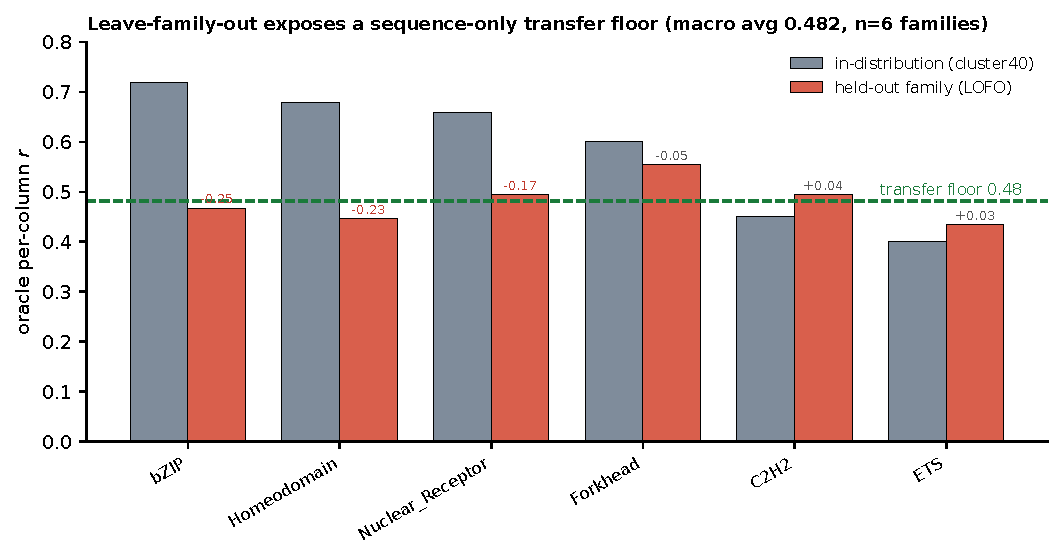
\includegraphics[width=0.85\linewidth]{figures/fig1g_lofo.pdf}
  \caption{\textbf{Leave-family-out transfer exposes a sequence-only floor.} Each structural family
  was held out entirely; TFScope was retrained on the remaining families and evaluated on the unseen
  family. Bars compare in-distribution (cluster40) and held-out (LOFO) oracle $r$ per family;
  numbers give the change. Families strong in-distribution collapse most (family memorization),
  families weak in-distribution hold or improve (transferable local features), and all converge
  toward a macro-average transfer floor (dashed).}
  \label{fig:lofo}
\end{figure} % NOTE: figure currently 6/8 families; regenerate scripts/build_lofo_figure.py after bHLH+Other finish

\subsection*{Distilling structural contacts is the principal accuracy lever}
We next asked why TFScope works, and traced its accuracy to a single, mechanistically interpretable
lever (Fig.~\ref{fig:fig2}a). Starting from the same training records DeepPBS uses, a sequence-only
model trained on that set alone reaches oracle $r$ 0.548 --- competent, but below structure-based
DeepPBS (0.626). Augmenting the corpus to 4{,}250 records lifts it to 0.596, closing most of the
data gap. The decisive step is contact distillation: adding the recognition-residue contact loss
(train-only, weight 0.3) lifts accuracy to 0.657, now above the structure-based method. The two
levers are complementary and neither alone suffices. Augmentation supplies breadth, but additional
PWM records saturate once the corpus is broad, because every PWM label encodes the same kind of
information --- the output of recognition. Contact distillation supplies something PWM labels never
contain: the geometry of which residues read which bases. In effect, the model is taught the
mechanism of recognition by structures during training and then reproduces specificity from
sequence, recovering through distillation the very signal that makes structure-based methods
accurate.

\subsection*{The sequence-only model recovers the protein--DNA recognition code}
If contact distillation genuinely transfers recognition physics, then the residues the model
treats as important should be the residues that actually read DNA. We tested this directly with an
in-silico alanine scan: mutating each DBD residue in turn and measuring how much the predicted PWM
changes yields a per-residue importance profile, which we compared against the DNA contacts
extracted geometrically from each test crystal structure --- contacts the model never sees at
training or inference (Fig.~\ref{fig:fig2}b). The agreement is strong and general: across the test
set, contacting residues are recovered above chance for the majority of factors (median per-TF
AUROC 0.65; 75\% above chance) and are 2.3-fold more important than other DBD positions
(Mann--Whitney $p\approx2\times10^{-46}$), with the result robust to excluding obligate dimers
whose basic regions might trivially dominate. The agreement is legible at the level of individual
proteins: for the C2H2 factor ZBTB7A the importance profile recovers five of six structural
contacts (AUROC 0.94), and for the homeodomain DUX4 it recovers six of twelve (AUROC 0.76).
Projected onto the three-dimensional complex, the model's hottest residues sit squarely on the
DNA interface (Fig.~\ref{fig:fig2}b). A model that was merely correlating sequence with motif
output would have no reason to concentrate its sensitivity on the physical contact residues; that
it does is evidence it has internalised recognition.

We then asked whether this importance corresponds to the recognition codes that structural biology
has established independently, using a structurally derived recognition-code resource
(rCLAMPS)~\cite{Wolfe2000,Najafabadi2015} as an external standard
(Fig.~\ref{fig:fig2}c). Aligning every test homeodomain to the canonical Pfam recognition
positions, TFScope's importance is sharply elevated at the true recognition residues (median
per-TF AUROC 0.69; 93\% above chance; recognition-position $z$=+0.62 against $-$0.05 elsewhere) ---
the model has, from sequence alone, rediscovered which residues of the homeodomain recognition
helix specify the bound base. The zinc-finger result is equally informative but for a different
reason: for C2H2 fingers the importance concentrates not on the canonical code positions
($z$=+0.11) but on the zinc-coordinating residues ($z$=+0.54). Biologically this is correct ---
the metal-ligating cysteines and histidines are the single most consequential residues for a zinc
finger, because without the folded $\beta\beta\alpha$ scaffold there is no recognition helix to
read DNA at all --- but it also identifies the long zinc-finger arrays as the honest frontier of
sequence-only prediction, where the dominant signal is scaffold integrity rather than a
transferable local code, consistent with these being the families on which the benchmark margin
favours structure. Finally, because the alanine-scan-plus-contact pipeline requires no
experimental structure of the target, it can be run prospectively: for in-distribution factors
that lack a solved complex we used AF3 folding and interface energetics to nominate plausible
recognition contacts (Fig.~\ref{fig:fig2}d), extending recognition-code annotation toward the
structureless majority of the proteome.

\subsection*{Proteome-scale nomination of motifs for orphan transcription factors}
Because TFScope needs only sequence, it can be turned on the dark proteome --- the factors that
have neither a solved complex nor a measured motif, and that are disproportionately developmental
regulators and disease genes. Across held-out factors, the sequence-only predictions recover
curated JASPAR/HOCOMOCO motifs~\cite{CastroMondragon2022} at per-gene median $r$=0.67, with 68\%
reaching $r\geq0.5$, and the accuracy falls off smoothly as DBD identity to the training set
declines (median identity 42\%; Fig.~\ref{fig:fig3}a). This smooth gradient, rather than a
threshold collapse, is the signature of genuine interpolation over sequence space: the model
extrapolates recognition from related factors rather than memorising specific motifs.

For orphan factors with no curated motif at all, we asked whether the nominated PWMs mark real
regulatory DNA in the genome (Fig.~\ref{fig:fig3}b,c). Scanning hg38 and comparing occupancy in
ENCODE candidate cis-regulatory elements against a dinucleotide-shuffle composition control --- a
control that is essential here, because it overturns a naive analysis confounded by GC content ---
five of six orphan nominations are significantly enriched in regulatory elements, with the
homeodomain factor ADNP2 enriched 17.5-fold at promoters and the germ-cell bHLH factor SOHLH1's
E-box enriched at enhancers. We interpret these as candidate-level functional plausibility rather
than measured occupancy, but they indicate that the nominated motifs are not statistical artefacts:
they fall preferentially in the regulatory compartments where the corresponding factors are
expected to act. Complementing this, model-guided in-silico optimisation of DNA toward maximal
predicted binding converges on each factor's consensus (Fig.~\ref{fig:fig3}d), showing that the
learned sequence-to-specificity map is invertible and specific, and can serve as a generative
oracle for designing or interpreting binding sites.

\subsection*{Sequence-only recovery of de novo designed DNA-binding proteins}
The most stringent test of whether a model has learned transferable recognition physics, rather
than the idiosyncrasies of natural protein families, is to confront it with proteins that have no
evolutionary history at all. We applied TFScope to four de novo computationally designed
helix--turn--helix DNA-binding proteins (DBP5, DBP6, DBP9, DBP35), each engineered to bind the
same target site (5$'$-GCAGATCTGCACATC-3$'$)~\cite{Glasscock2025}, and compared its predicted
motifs against the experimental binding landscape these proteins were characterised with --- the
relative binding measured for every single base-pair substitution by yeast-display competition
(Fig.~\ref{fig:fig3}e). From sequence alone, TFScope recovers the central CAC recognition core of
these designed proteins, and --- more tellingly --- does so with a confidence that tracks the
experimental signal. For DBP6 the predicted high-information CAC sits exactly over the columns the
mutation scan identifies as most specificity-determining (per-position agreement 83\%, $r$=0.65),
whereas DBP5, DBP9 and DBP35 are recovered partially ($r$=0.39--0.59; mean across designs 0.53).
The result is therefore not all-or-nothing but a calibrated, graded prediction: TFScope is
confident and correct where the designed interface makes a strong, natural-like major-groove
contact, and appropriately tentative where it does not. Consistent with a purely sequence-based
readout, the flanking positions carry little predicted information --- sensible for DNA the scaffold
does not specifically contact --- whereas the shape-driven, minor-groove flank preferences that a
structure-based method can infer from the designed backbone are, by construction, beyond a
sequence-only model. That a model trained only on natural TFs nonetheless reads the specificity of
proteins designed from scratch is strong evidence that it has learned the physics of major-groove
recognition rather than the memorised motifs of any family, and it suggests a concrete role for
TFScope in protein design: a rapid, structure-free filter for which designed binders have
confidently predictable specificity before committing to structural modelling or wet-lab
characterisation.

\subsection*{A sequence-to-structure hybrid predicts mutational effects on specificity}
A specificity model is most useful clinically when it can predict how a mutation changes
recognition, since such mutations underlie both natural specificity evolution and disease.
We tested this on a textbook case --- the myogenic bHLH master regulator MyoD, whose basic-region
substitution L122R is known to shift its preference from the myogenic E-box CACCTG toward the
canonical MYC-like CACGTG~\cite{Ma1994} --- and quantified the effect with a directional
difference-in-differences switch score rather than a brittle consensus comparison, because the
single most-probable base of a predicted PWM is unstable to small perturbations
(Fig.~\ref{fig:fig4}a). From sequence alone, TFScope reproduces the switch: the wild-type DBD
strongly prefers the myogenic E-box ($S_{\mathrm{CACGTG}}-S_{\mathrm{CACCTG}}=-11.8$), whereas
L122R raises the CACGTG score from $-0.4$ to $+5.8$ and collapses the preference gap to $-2.6$,
yielding a switch score of $+9.2$ --- the predicted preference moves unambiguously in the
documented direction, a shift a consensus-only readout would have missed because the mutant's
single top base does not by itself flip. The model's sensitivity, moreover, scales with the size
of the determinant change: titrating the nuclear-receptor P-box and recognition module shows that
single residues and the three-residue P-box perturb but do not redirect the predicted motif,
whereas swapping the bulk of the recognition module crosses the resolved threshold at 50--75\% of
differing residues (Fig.~\ref{fig:fig4}a). TFScope therefore captures specificity at the level of
the recognition module --- the unit at which evolution actually rewires DNA binding --- rather than
of isolated de-novo substitutions.

Where sequence localises the affected position but cannot name the exact new base, a targeted
structure step calibrates it, and the two methods combine into a clean division of labour
(Fig.~\ref{fig:fig4}b,c). For MyoD L122R, TFScope correctly flags the central E-box position as
the one that changes but assigns the wrong de-novo base (predicting CAC\textbf{A}TG against the true
CAC\textbf{G}TG). To resolve the base we refolded the bHLH homodimer on each candidate E-box with
AlphaFold3 (five models per base) and scored the protein--DNA interface energy with Rosetta. By
ensemble median, the true switch CACGTG ranks best ($-$25.9 REU), the wild-type CACCTG second
($-$24.9), and TFScope's CACATG decisively worst ($-$13.3) --- so the structure step calibrates the
sequence-only error A$\to$G, and an independent structural readout (DeepPBS on the same dimer) also
recovers G. Two control analyses establish why this works and how to do it correctly, and both have
a biophysical reading. First, the per-candidate \emph{refold} is essential: simply mutating the
base in a fixed backbone (an in-place scan) is dominated by steric clash and fails to recover G,
because recognition is an induced-fit process in which the protein adapts its conformation to the
base it reads; only by letting each candidate base be modelled with its own relaxed complex is the
true preference revealed. Second, the calibration must be read from the structural \emph{ensemble},
not a single model, because the per-model interface energy is noisy and, tellingly, the structure
predictor's own confidence is uniform across all four bases --- the predictor folds the wrong base
just as confidently as the right one, so it is the interface energetics, not the structure
predictor, that discriminate. The resulting hybrid is therefore complementary rather than
competitive: sequence localises and scales across the proteome, and a lightweight,
TFScope-targeted structure calculation resolves the atomic identity of a de-novo base where it
matters.

% ─────────────────────────────────────────────────────────────────────────────
\section*{Discussion}

TFScope establishes that the information needed to predict transcription-factor DNA-binding
specificity is present in protein sequence, and that it can be extracted to match the
structure-based state of the art without any structure at inference. The key idea is that a PWM
label records the outcome of recognition but not its mechanism, and that the missing mechanistic
signal --- which residues contact which bases --- can be distilled from structures during training
and thereafter reproduced from sequence. Several conclusions follow with implications beyond the
specific model.

First, decoupling specificity prediction from structure determination changes what is annotatable.
Because TFScope requires only an amino-acid sequence, it can be applied to every human TF and to
the orthologues, paralogues, splice products, designed proteins, and disease variants for which
docked complexes will never exist --- precisely the dark proteome where the need is greatest. The
smooth decline of accuracy with sequence divergence, the enrichment of orphan nominations in
cis-regulatory elements, and the recovery of de-novo designed proteins together indicate that this
reach is real rather than nominal, with the zinc-finger arrays marking an honest ceiling.

Second, the accuracy is mechanistically interpretable, which matters for a method intended to guide
biology. The model's importance localises to the residues structural biology has long known to read
DNA, recovering the homeodomain recognition positions and respecting the dependence of zinc-finger
recognition on metal coordination. In this sense TFScope does not merely predict motifs; it
recapitulates, from sequence, a recognition code that took decades of crystallography and
biochemistry to assemble --- and it does so across families rather than within one. This offers a
route to extend recognition-code reasoning to the many factors and engineered proteins for which no
code has been derived.

Third, sequence and structure are complementary, not competing. Sequence-only prediction is
weakest exactly where recognition is a property of quaternary assembly or multi-domain
combinatorics --- dimeric basic-region factors and long zinc-finger arrays --- and it cannot, on its
own, name the new base created by a de-novo mutation. A lightweight sequence$\to$structure hybrid
resolves both: TFScope localises and scales, and a targeted structure calculation supplies atomic
resolution where, and only where, it is needed. The induced-fit requirement we uncover in the
calibration --- that each candidate base must be modelled with its own relaxed complex --- is itself
a reminder that protein--DNA recognition is a conformationally coupled process, and that scoring a
mutation in a fixed backbone misrepresents it.

The limitations are specific and delineate where the field should push next. Specificity that
depends on dimerisation register or on the combinatorial arrangement of many domains is
under-determined by a single chain, and is where structure retains a clear advantage; the orphan
nominations are functional-plausibility candidates rather than measured occupancy; the benchmark
margin over the structure-based method, though supported by significance testing and the baseline
ladder, is modest; and we find that structural family labels are themselves motif-incoherent --- a
single structural family maps to many distinct motif grammars --- which is why TFScope conditions on
learned rather than label-derived family features and why naive family supervision does not help.
Natural extensions include oligomer-aware inputs that present the assembled binding unit, richer
forms of contact distillation that capture shape as well as base-specific readout, and coupling to
genome-scale occupancy data so that predicted specificity can be reconciled with measured binding.
By making specificity prediction a property of sequence rather than of structure, TFScope turns an
annotation that was available for a privileged few factors into one that can, in principle, be
computed for the entire regulatory proteome.

% ─────────────────────────────────────────────────────────────────────────────
\section*{Methods}

\noindent\textbf{Data curation and family assignment.} We combined a curated augmentation corpus
with the DeepPBS training records (4{,}250 PWM records), trimmed each protein to a canonical DBD,
and canonicalised PWMs; family assignments use a learned 10-class scheme (alternatives: rebin-34,
famv2-46, coarse-12)~\cite{Weirauch2014,CastroMondragon2022,Fornes2020}.

\noindent\textbf{Splits and contamination control.} The primary split (cluster40) clusters factors
at 40\% DBD identity~\cite{LiGodzik2006} so that no test factor exceeds that identity to training;
we additionally report the DeepPBS 130-TF blind split. Structure-level splitting leaks
near-duplicate complexes and inflates all methods, motivating cluster40.

\noindent\textbf{Model architecture.} Let a TF be a sequence $x=(x_1,\dots,x_L)$ of $L$ residues.
An ESM-2 (650\,M)~\cite{Lin2023} encoder with low-rank adapters~\cite{Hu2022} produces contextual
embeddings $H=\mathrm{ESM2}_{\mathrm{LoRA}}(x)\in\mathbb{R}^{L\times d}$ with rows $h_i$. A learned
pooling gate scores each residue and pools the DNA-binding domain by a gate-weighted average,
\begin{equation}
g_i=\sigma\!\big(w_g^{\top}h_i+b_g\big),\qquad
z=\frac{\sum_{i=1}^{L} g_i\,h_i}{\sum_{i=1}^{L} g_i}\in\mathbb{R}^{d},
\end{equation}
so that disordered and linker residues, which carry no base specificity, are down-weighted. A
family-conditioned mixture-of-experts decoder then conditions $z$ on the structural-class embedding
$e_f$ via FiLM modulation and a soft routing over $E$ experts,
\begin{equation}
\alpha=\mathrm{softmax}\!\big(W_r[z;e_f]\big)\in\Delta^{E-1},\qquad
u=\underbrace{f_{\mathrm{sh}}(z)}_{\text{shared}}+\sum_{e=1}^{E}\alpha_e\,f_e\!\big(\gamma_f\odot z+\beta_f\big),
\end{equation}
with SwiGLU experts $f_e$ and FiLM parameters $(\gamma_f,\beta_f)$ predicted from $e_f$. A
cross-attention head with $W$ learned motif-position queries $Q\in\mathbb{R}^{W\times d}$ attends to
the residue keys/values $(K,V)=(HW_K,HW_V)$ conditioned on $u$, producing per-column base logits
$\ell\in\mathbb{R}^{4\times W}$, from which the predicted PWM and the motif-core gate are
\begin{equation}
A=\mathrm{softmax}\!\Big(\tfrac{QK^{\top}}{\sqrt{d}}\Big)\in\mathbb{R}^{W\times L},\qquad
P_{b,j}=\frac{\exp(\ell_{b,j})}{\sum_{b'=1}^{4}\exp(\ell_{b',j})},\qquad
\hat{\gamma}_j=\sigma\!\big(w_\gamma^{\top}\,(AV)_j\big),
\end{equation}
where $P\in\mathbb{R}^{4\times W}$ is the position weight matrix over $\{$A,C,G,T$\}$ and
$\hat\gamma_j\in[0,1]$ marks active motif columns. The row of $A$ summed over query columns,
$\bar a_i=\sum_j A_{j,i}$, gives the attention mass placed on residue $i$ and is the quantity
supervised by structural contacts.

\noindent\textbf{Training objective.} The model is trained by minimising a composite loss whose
principal terms compare the predicted PWM $P$ and gate $\hat\gamma$ with the canonicalised target
$(P^\star,\gamma^\star)$ over the target columns $\mathcal{M}$, and align the residue attention
$\bar a$ with the recognition-residue contact target $c^\star\in\{0,1\}^{L}$:
\begin{align}
\mathcal{L}_{\mathrm{pwm}}&=\sum_{j\in\mathcal{M}}\sum_{b=1}^{4}\big|P_{b,j}-P^\star_{b,j}\big|,
&\mathcal{L}_{\mathrm{gate}}&=\mathrm{BCE}\big(\hat\gamma,\gamma^\star\big),\nonumber\\
\mathcal{L}_{\mathrm{contact}}&=\mathrm{BCE}\big(\bar a,\,c^\star\big),
&\mathcal{L}_{\mathrm{IC}}&=\big|\,\mathrm{IC}(P)-\mathrm{IC}(P^\star)\,\big|+\big(1-\rho_{\mathrm{IC}}\big),
\end{align}
where $\mathrm{IC}(P)_j=2+\sum_b P_{b,j}\log_2 P_{b,j}$ and $\rho_{\mathrm{IC}}$ is the Pearson
correlation between the predicted and target per-column information content. With a Switch-style
load-balancing term $\mathcal{L}_{\mathrm{bal}}$ and an expert-diversity term
$\mathcal{L}_{\mathrm{div}}$, the total objective is
\begin{equation}
\mathcal{L}=\lambda_{\mathrm{pwm}}\mathcal{L}_{\mathrm{pwm}}
+\lambda_{\mathrm{gate}}\mathcal{L}_{\mathrm{gate}}
+\lambda_{\mathrm{con}}\mathcal{L}_{\mathrm{contact}}
+\lambda_{\mathrm{IC}}\mathcal{L}_{\mathrm{IC}}
+\lambda_{\mathrm{bal}}\mathcal{L}_{\mathrm{bal}}
+\lambda_{\mathrm{div}}\mathcal{L}_{\mathrm{div}},
\end{equation}
with $(\lambda_{\mathrm{pwm}},\lambda_{\mathrm{gate}},\lambda_{\mathrm{con}},\lambda_{\mathrm{IC}},
\lambda_{\mathrm{bal}},\lambda_{\mathrm{div}})=(1.0,1.0,0.3,0.5,0.05,0.01)$. The contact target
$c^\star$ is a recognition-residue prior derived only from the cluster40 \emph{training} partition;
it enters solely through $\mathcal{L}_{\mathrm{contact}}$ at training time, and no structural input
is used at inference ($P,\hat\gamma$ are functions of $x$ alone). Optimisation used AdamW with
global batch 36, learning rate $4.5\times10^{-4}$, for 225 epochs.

\noindent\textbf{Evaluation.} The primary metric is the oracle-aligned per-column Pearson $r$.
Writing $P^{(\delta,s)}$ for the predicted PWM shifted by offset $\delta$ on strand
$s\in\{+,-\}$ (the $-$ strand applying a reverse-complement), and $\mathcal{C}$ for the set of
target core columns (information content $\geq0.25$), the alignment and score are
\begin{equation}
(\delta^\star,s^\star)=\!\!\argmax_{|\delta|\leq 10,\,s}\ \frac{1}{|\mathcal{C}|}\!\sum_{j\in\mathcal{C}}\!
\mathrm{corr}\!\big(P^{(\delta,s)}_{:,j},P^\star_{:,j}\big),\qquad
r=\frac{1}{|\mathcal{C}|}\sum_{j\in\mathcal{C}}\mathrm{corr}\!\big(P^{(\delta^\star,s^\star)}_{:,j},P^\star_{:,j}\big).
\end{equation}
The identical alignment is applied symmetrically to all methods, DeepPBS included, so that no method
is advantaged by motif placement. Supporting metrics include per-position $r$, mean absolute error
over $[0,2]$ (as in DeepPBS), top-1 (argmax) base accuracy, and KL divergence; significance uses
paired bootstrap and Wilcoxon signed-rank tests. The score of a candidate site $s=(s_1,\dots,s_k)$
under a predicted PWM, used in the mutation and design analyses, is the best log-odds against a
uniform background over offsets $o$ and strands,
\begin{equation}
S(s)=\max_{o,\ \mathrm{strand}}\ \sum_{k} \log_2\!\frac{P_{s_k,\,o+k}}{0.25}.
\end{equation}

\noindent\textbf{Baselines.} Random (shuffled-column, dinucleotide-matched), NN-PWM (leave-gene-out
nearest DBD by ESM-2 cosine, copy donor PWM), a frozen-ESM-2 linear regressor, and the DeepPBS
ensemble~\cite{Mitra2024}.

\noindent\textbf{Structural plausibility (AF3 consensus folding).} For each test TF we folded the
protein with its predicted highest-IC consensus oligo (TFScope and DeepPBS separately, correct
oligomer state) using AlphaFold3~\cite{Jumper2021} and compared interface ipTM and pLDDT, paired
per-TF.

\noindent\textbf{In-silico mutagenesis and recognition-code comparison.} Single-residue alanine
scans quantify per-residue importance as the L1 change in the predicted PWM. Geometric DNA contacts
(protein atoms within 4.5\,\AA{} of a DNA base atom) extracted from test crystal structures provide
training-independent labels; recognition-code positions are taken from a structural
recognition-code resource (rCLAMPS)~\cite{Wolfe2000,Najafabadi2015}.

\noindent\textbf{Genome-wide motif scanning.} MOODS scans of hg38 ($p<10^{-4}$, both strands)
against ENCODE candidate cis-regulatory elements, with a dinucleotide-shuffle composition control.

\noindent\textbf{Mutation switch score.} For a predicted PWM and an E-box $s$, $S(s)$ is the best
log-odds of $s$ over offsets and strands; the directional switch score is
$\Delta_{\text{switch}}=[S_{\text{mut}}(\text{CACGTG})-S_{\text{mut}}(\text{CACCTG})]-
[S_{\text{WT}}(\text{CACGTG})-S_{\text{WT}}(\text{CACCTG})]$.

\noindent\textbf{Designed-protein evaluation.} The four designed proteins and their
single-base-pair binding data are from the design study~\cite{Glasscock2025}. At position $p$ with
wild-type base $w_p$, the experimental relative binding of base $b$ and TFScope's predicted relative
preference are, respectively,
\begin{equation}
E_{b,p}=\log_2\!\frac{v_{b,p}}{v_{w_p,p}},\qquad
\hat E_{b,p}=\log_2\!\frac{P_{w_p,p}}{P_{b,p}},
\end{equation}
where $v_{b,p}$ is the normalised median PE/FITC signal (lower $=$ stronger binding, so both
quantities are negative when $b$ binds more strongly than wild type). Agreement over the aligned
core is reported as the column-wise Pearson correlation between $\hat E$ and $E$ and as the
per-position argmax agreement.

\noindent\textbf{Structure calibration of mutant bases.} For each candidate base $b$ at the mutated
position, AlphaFold3 refolds the mutant DBD as its biological oligomer on the corresponding site,
producing $M{=}5$ models $\{m\}$; each complex is relaxed and its protein--DNA interface energy
$E_{\mathrm{int}}$ is computed with Rosetta (\texttt{pwm\_hybrid}, FastRelax, beta\_nov16/RM8B
charges). Candidates are ranked by the ensemble-median interface energy relative to the seeded base,
\begin{equation}
\Delta\Delta G(b)=\operatorname*{median}_{m=1}^{M}\Big[E_{\mathrm{int}}^{(m)}(b)-E_{\mathrm{int}}^{(m)}(b_0)\Big],
\qquad b^\star=\argmin_{b}\ \Delta\Delta G(b),
\end{equation}
the median (rather than the mean or a single model) being used because the per-model relaxed energy
is heavy-tailed. The per-candidate refold is required: scoring $b$ in a fixed backbone instead of
$E_{\mathrm{int}}^{(m)}(b)$ is dominated by steric clash and does not recover $b^\star$.

% ─────────────────────────────────────────────────────────────────────────────
\section*{Data and code availability}
DeepPBS benchmark data are from the original publication~\cite{Mitra2024}; CIS-BP and
JASPAR~\cite{Weirauch2014,CastroMondragon2022} are publicly available; designed-protein data are
from~\cite{Glasscock2025}. The augmented dataset, splits, source code, and trained checkpoints will
be released upon acceptance.

% ─────────────────────────────────────────────────────────────────────────────
\bibliographystyle{unsrtnat}
\bibliography{refs}

% ─────────────────────────────────────────────────────────────────────────────
\clearpage
\begin{figure}[p]\centering
  \begin{subfigure}{0.93\linewidth}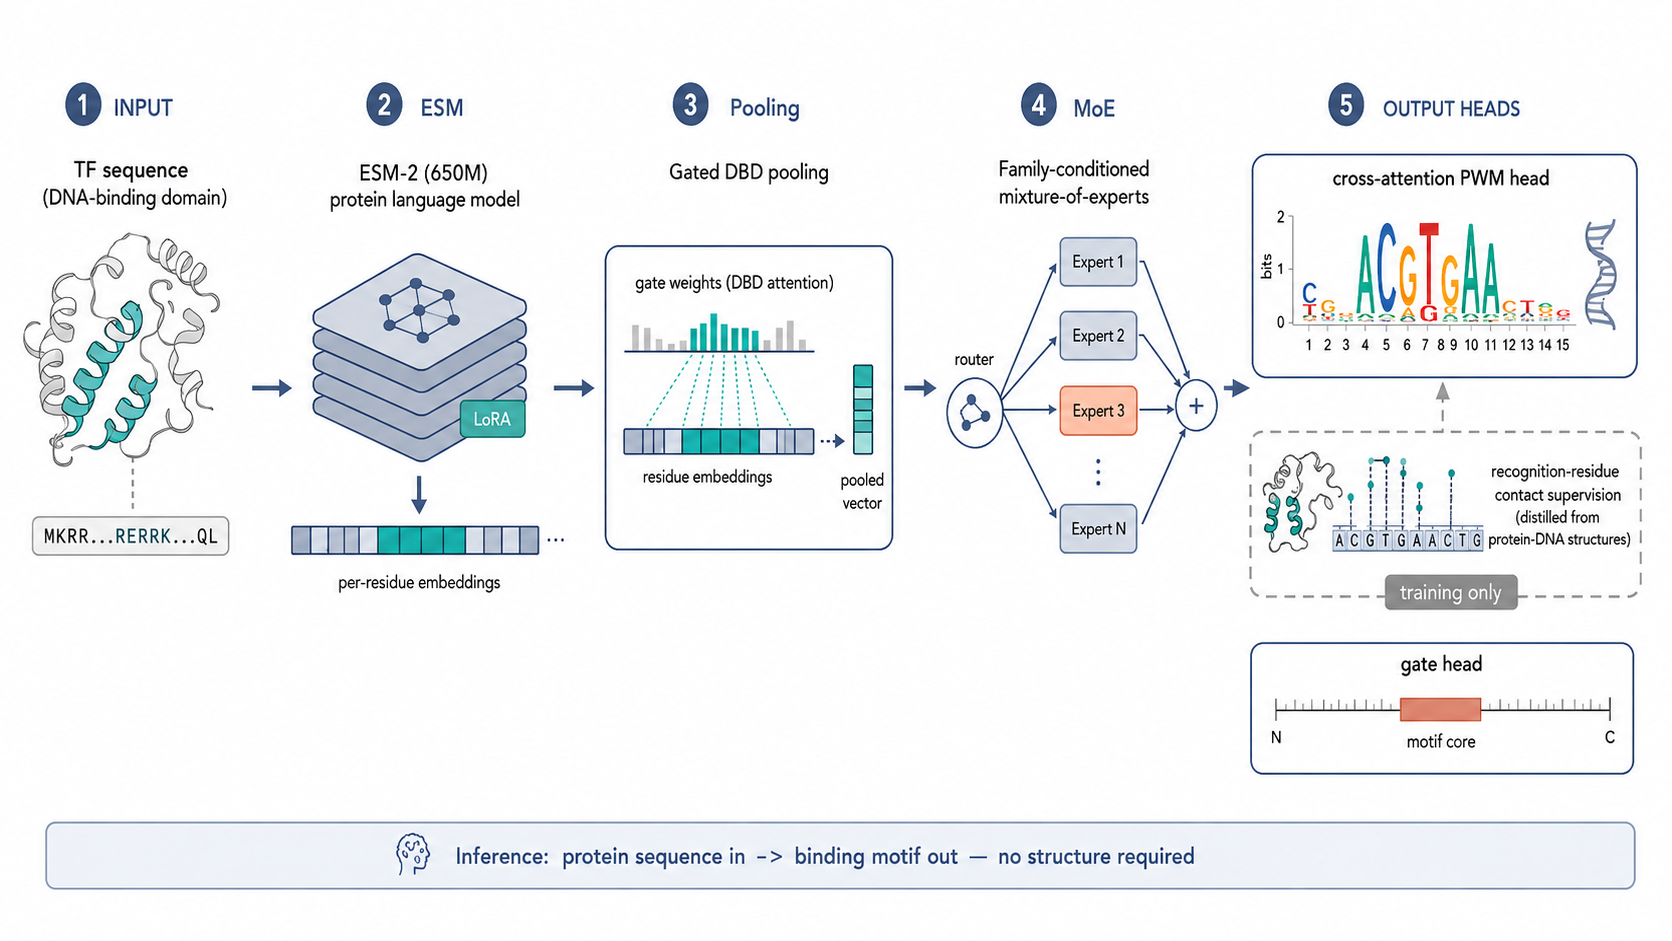
\includegraphics[width=\linewidth]{figures/fig1a_architecture.png}\caption{}\end{subfigure}\\[4pt]
  \begin{subfigure}{0.46\linewidth}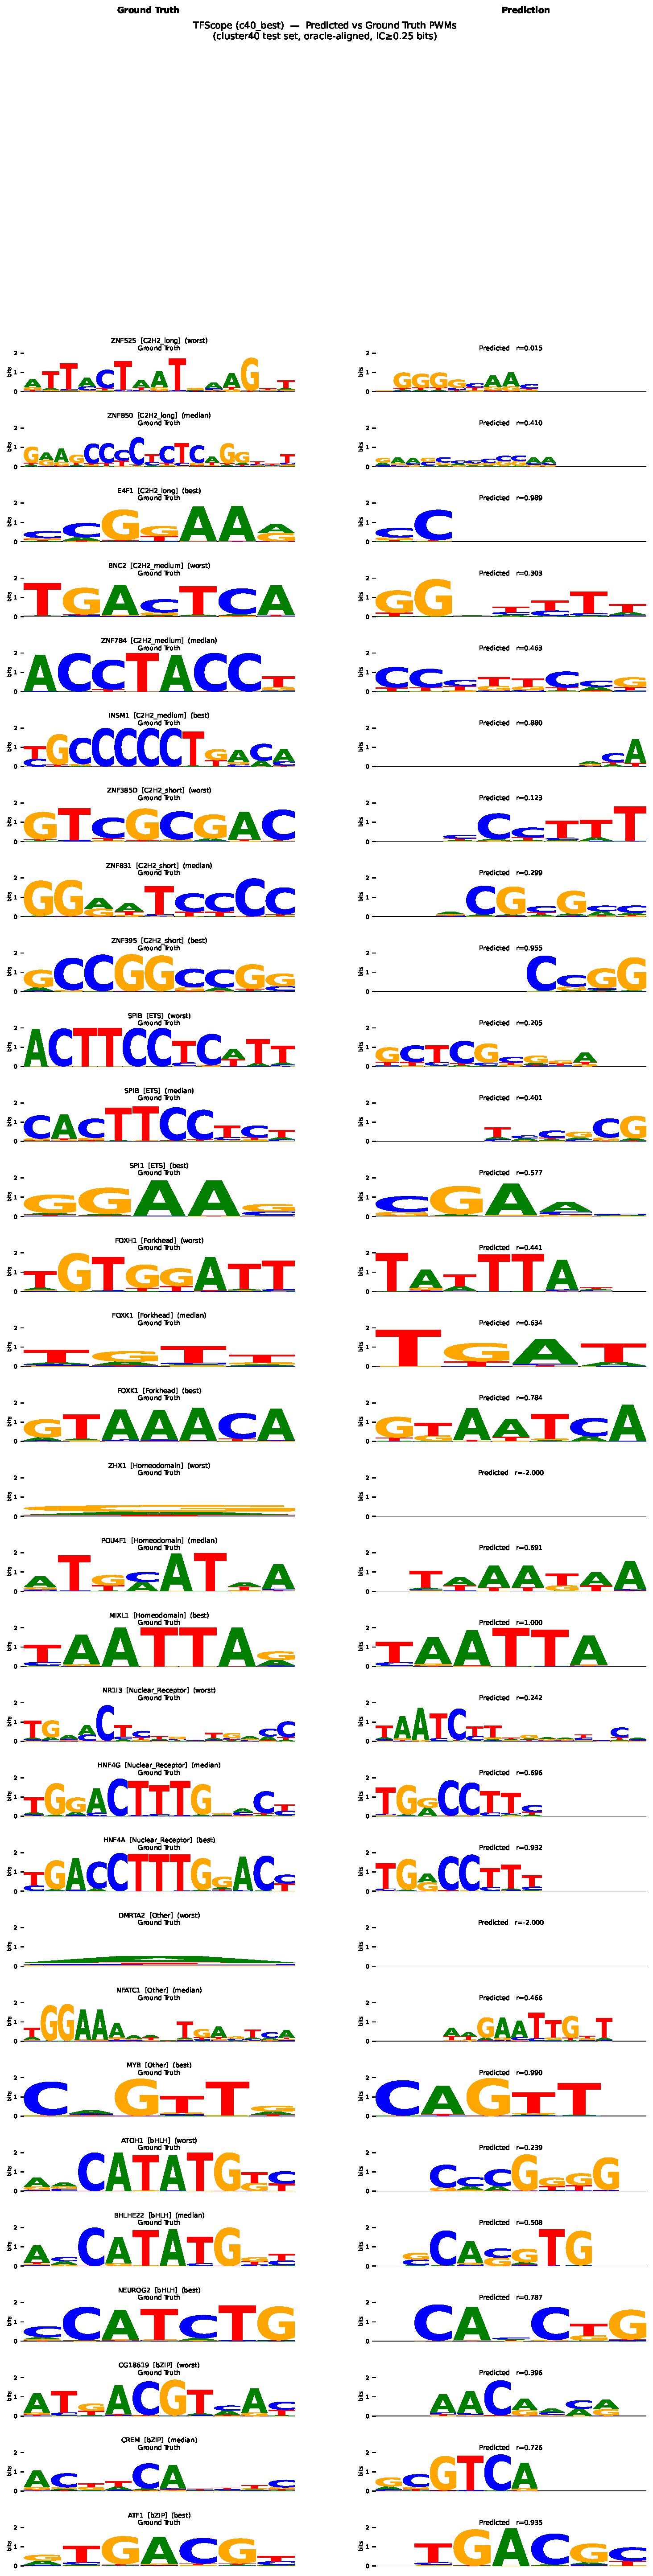
\includegraphics[width=\linewidth]{figures/fig1bc_benchmark.pdf}\caption{}\end{subfigure}\hfill
  \begin{subfigure}{0.46\linewidth}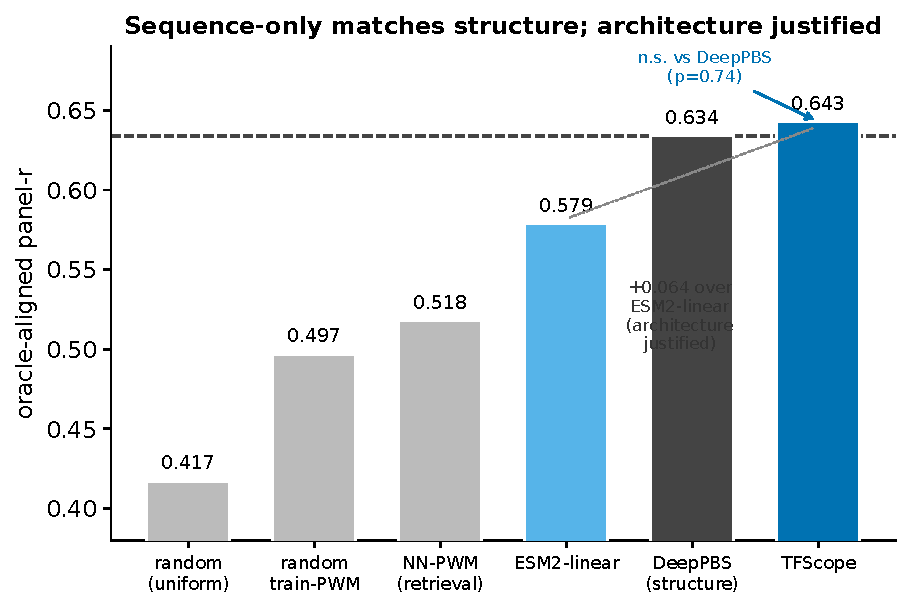
\includegraphics[width=\linewidth]{figures/fig1d_baseline_ladder.pdf}\caption{}\end{subfigure}\\[4pt]
  \begin{subfigure}{0.46\linewidth}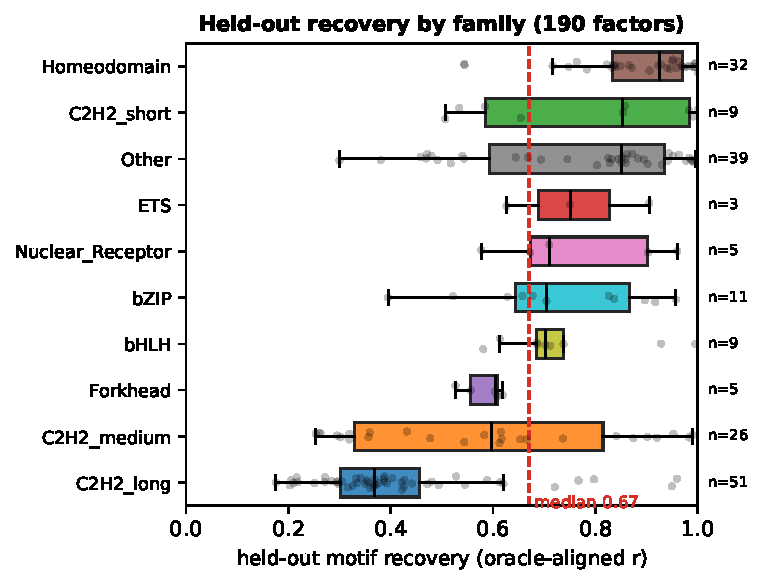
\includegraphics[width=\linewidth]{figures/fig1e_perfamily.pdf}\caption{}\end{subfigure}\hfill
  \begin{subfigure}{0.46\linewidth}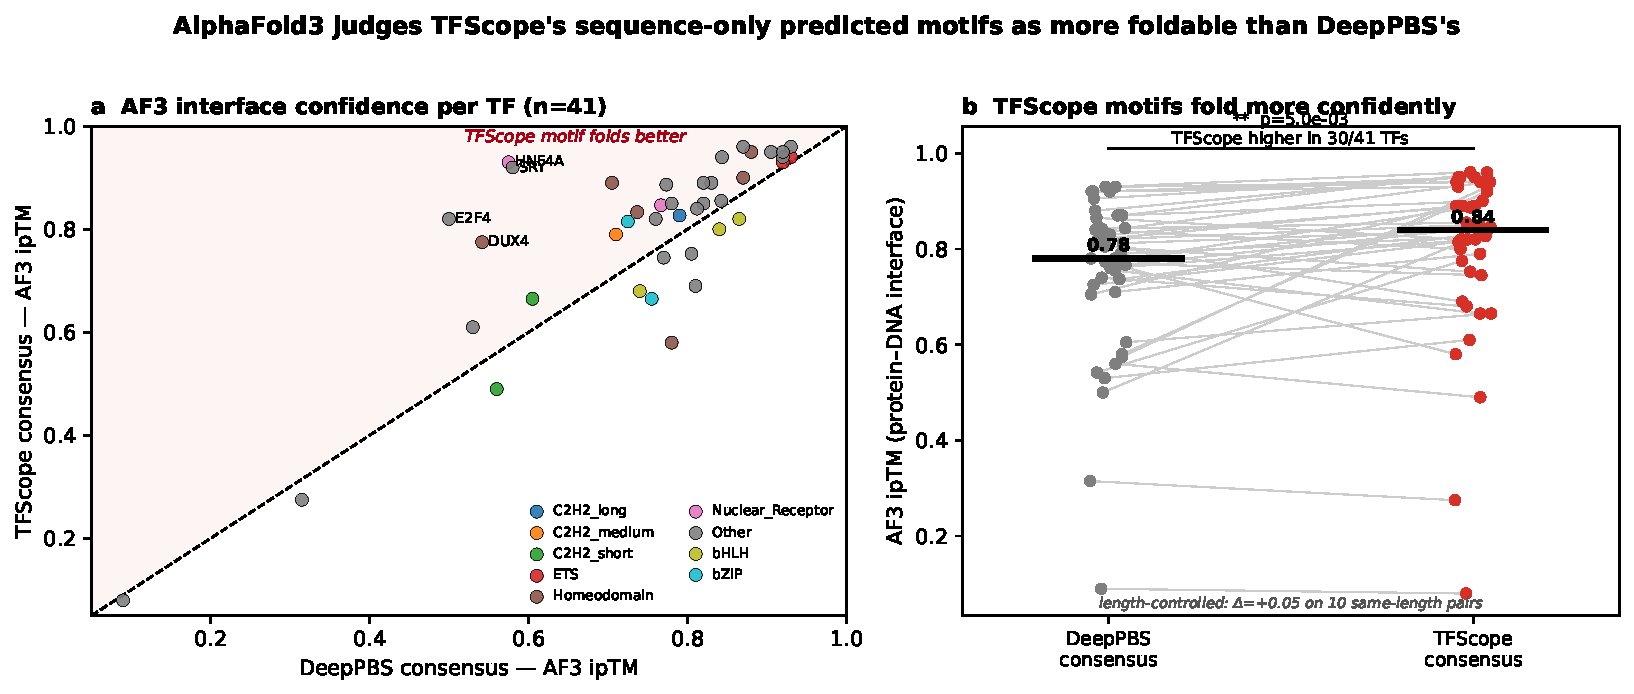
\includegraphics[width=\linewidth]{figures/fig1f_foldability.pdf}\caption{}\end{subfigure}
  \caption{\textbf{Structure-free prediction matches structure-based specificity.}
  (a) TFScope architecture: ESM-2/LoRA encoder $\to$ gated DBD pooling $\to$ family-conditioned
  mixture-of-experts $\to$ cross-attention PWM head; recognition-residue contact supervision is
  applied only at training, inference is sequence-only. (b,c) On the contamination-controlled
  cluster40 hold-out, TFScope (oracle $r$ 0.657) matches DeepPBS (0.626) without structure.
  (d) Baseline ladder (mean oracle $r$): random 0.464, NN-PWM 0.534, frozen-ESM-2 linear 0.555,
  DeepPBS 0.626, TFScope 0.657 (TFScope$-$DeepPBS $p$=0.30; TFScope$-$linear $+$0.102).
  (e) Per-family accuracy vs.\ DeepPBS: TFScope wins ``Other''/NR/bHLH, DeepPBS wins
  bZIP/long-C2H2. (f) AF3 interface confidence of complexes built from each method's predicted
  consensus ($n$=41): TFScope ipTM 0.795 vs.\ DeepPBS 0.744 (Wilcoxon $p$=5$\times$10$^{-3}$).}
  \label{fig:fig1}
\end{figure}

\begin{figure}[p]\centering
  \begin{subfigure}{0.49\linewidth}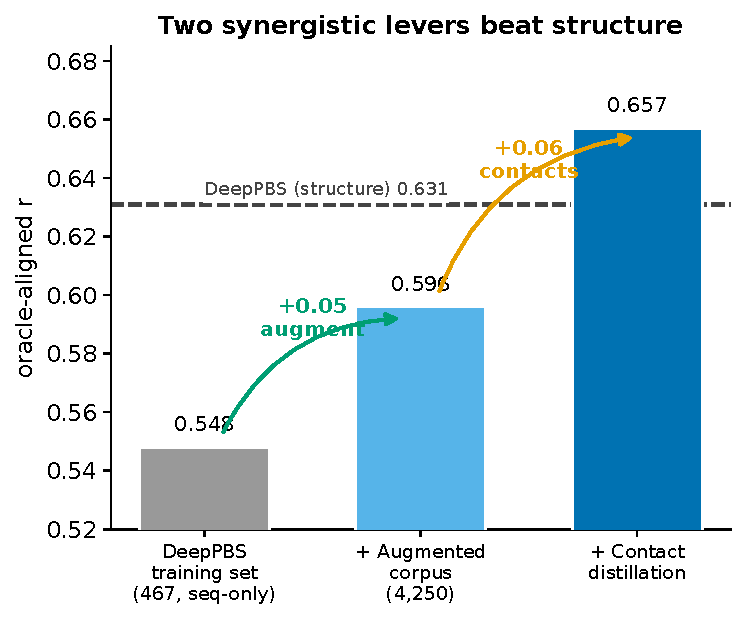
\includegraphics[width=\linewidth]{figures/fig2a_ablation.pdf}\caption{}\end{subfigure}\hfill
  \begin{subfigure}{0.49\linewidth}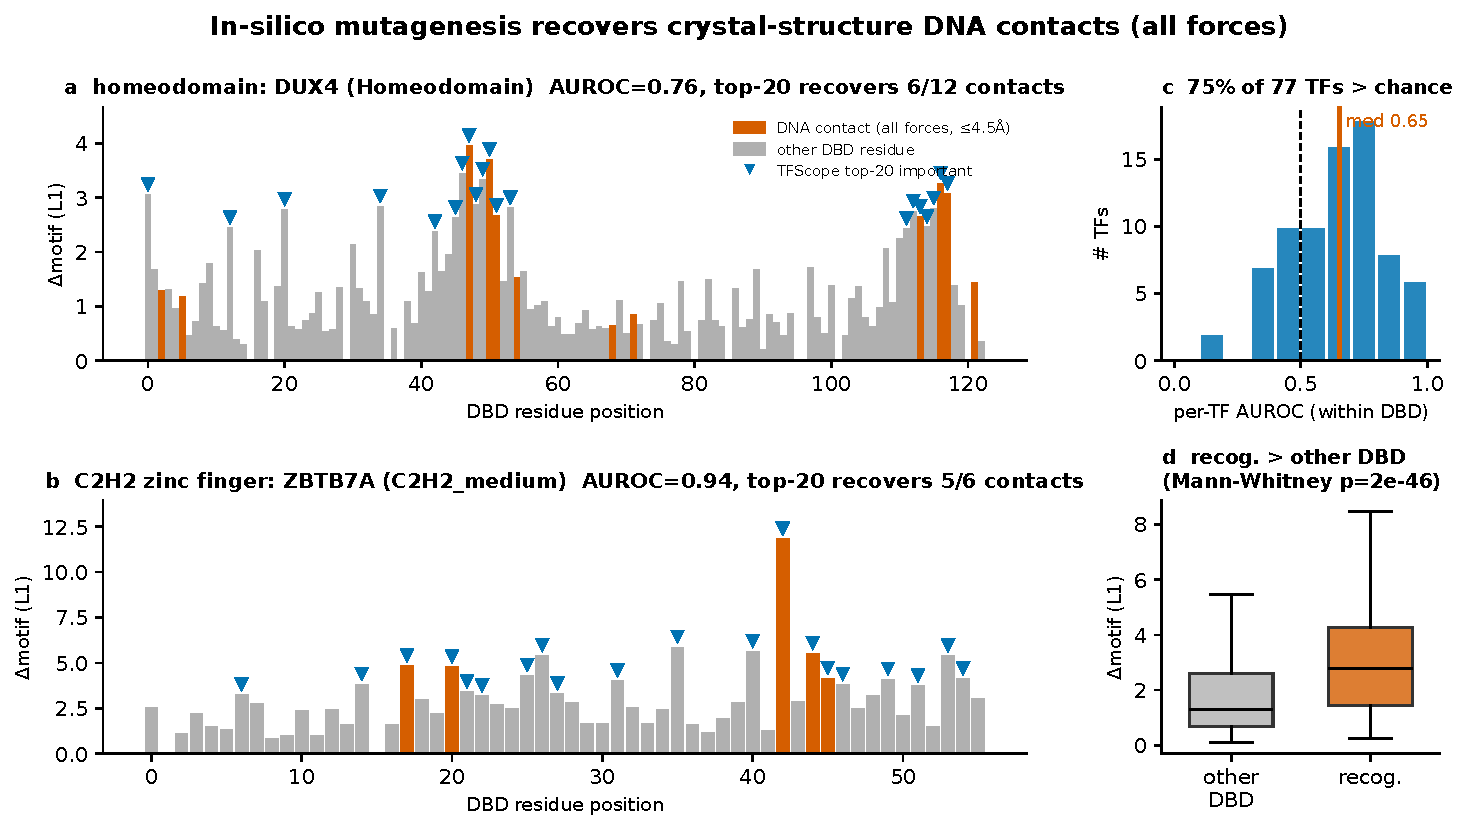
\includegraphics[width=\linewidth]{figures/fig2b_mutagenesis.pdf}\caption{}\end{subfigure}\\[4pt]
  \begin{subfigure}{0.49\linewidth}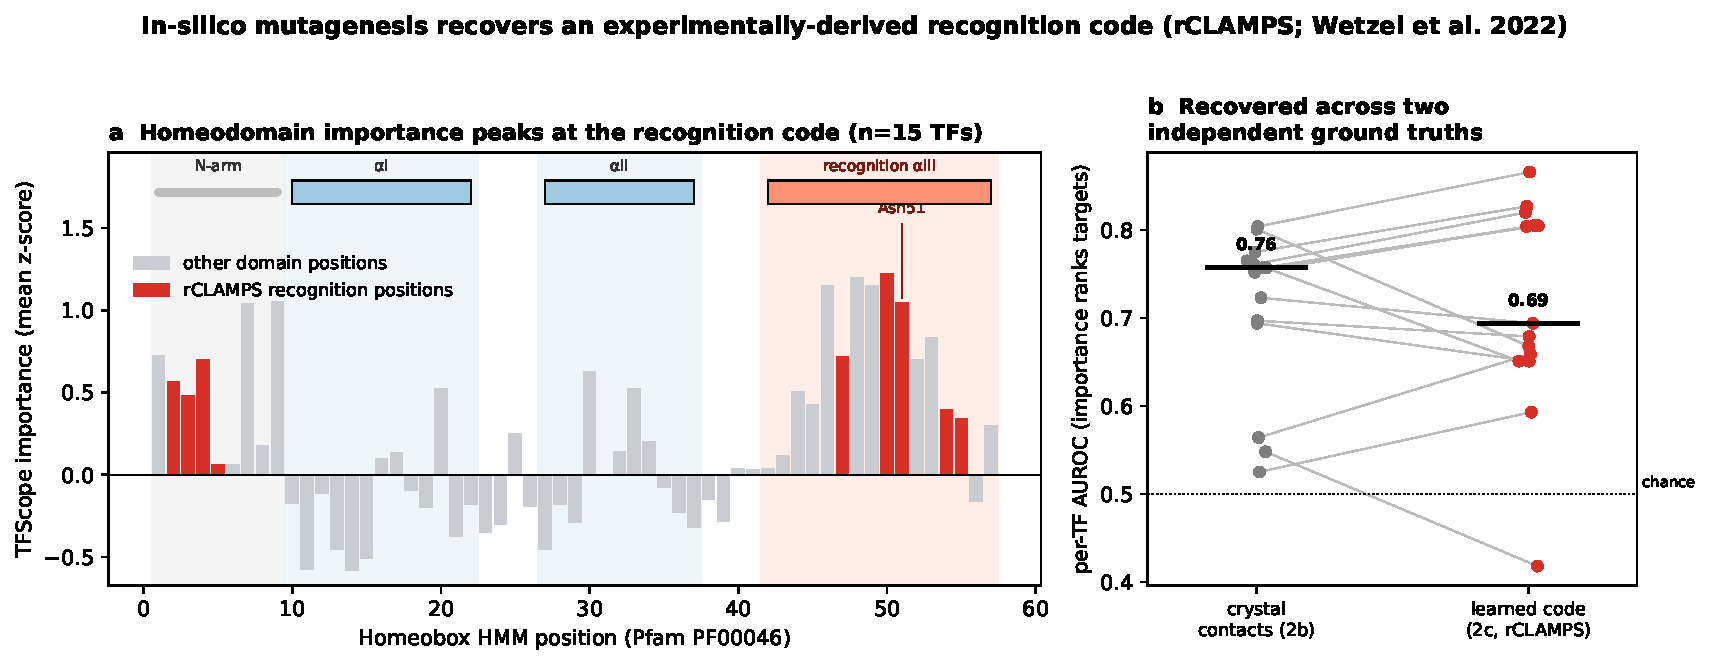
\includegraphics[width=\linewidth]{figures/fig2c_recognition.pdf}\caption{}\end{subfigure}\hfill
  \begin{subfigure}{0.49\linewidth}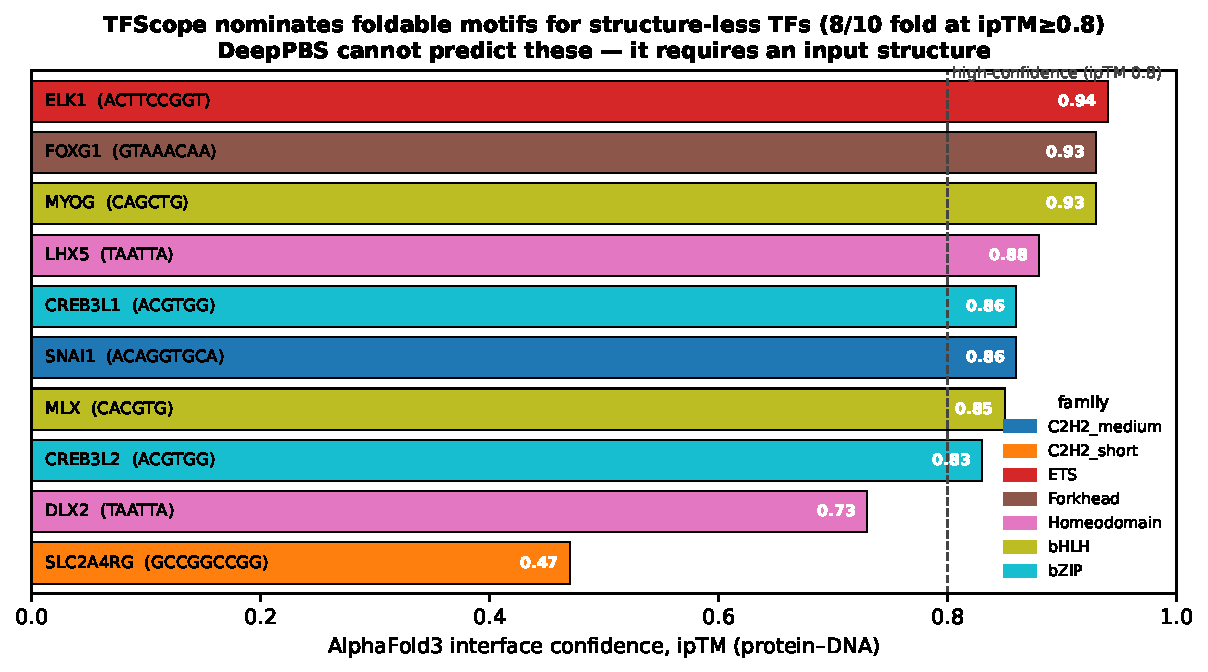
\includegraphics[width=\linewidth]{figures/fig2d_structureless.pdf}\caption{}\end{subfigure}
  \caption{\textbf{Contact distillation drives accuracy and recovers the recognition code.}
  (a) Two levers carry the sequence-only model past structure: DeepPBS-train-only 0.548 $\to$
  corpus augmentation 0.596 $\to$ recognition-contact distillation 0.657 (DeepPBS 0.626).
  (b) In-silico alanine-scan importance recovers structure-derived DNA contacts (population median
  AUROC 0.65; contacts 2.3$\times$ more important; examples ZBTB7A 0.94, DUX4 0.76) and maps onto
  the DNA interface. (c) Importance is elevated at experimentally derived homeodomain recognition
  positions (median AUROC 0.69; recognition $z$=+0.62 vs.\ $-$0.05); for C2H2 fingers it
  concentrates on zinc-coordinating residues ($z$=+0.54). (d) For structure-less TFs, AF3 folding
  plus interface energetics nominate plausible recognition contacts.}
  \label{fig:fig2}
\end{figure}

\begin{figure}[p]\centering
  \begin{subfigure}{0.49\linewidth}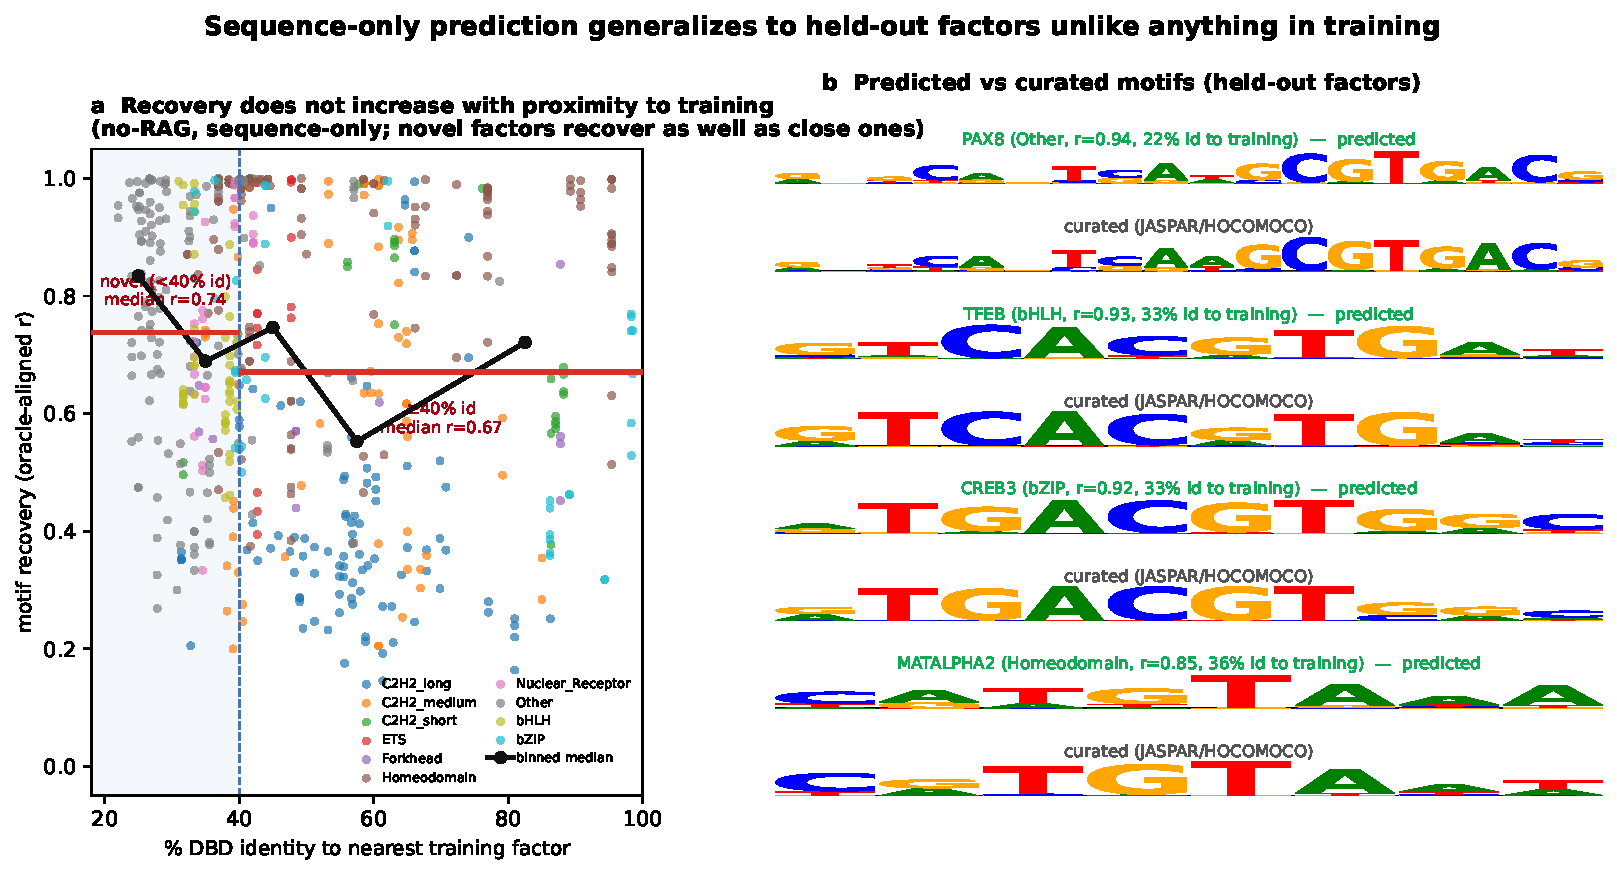
\includegraphics[width=\linewidth]{figures/fig3a_recovery.pdf}\caption{}\end{subfigure}\hfill
  \begin{subfigure}{0.49\linewidth}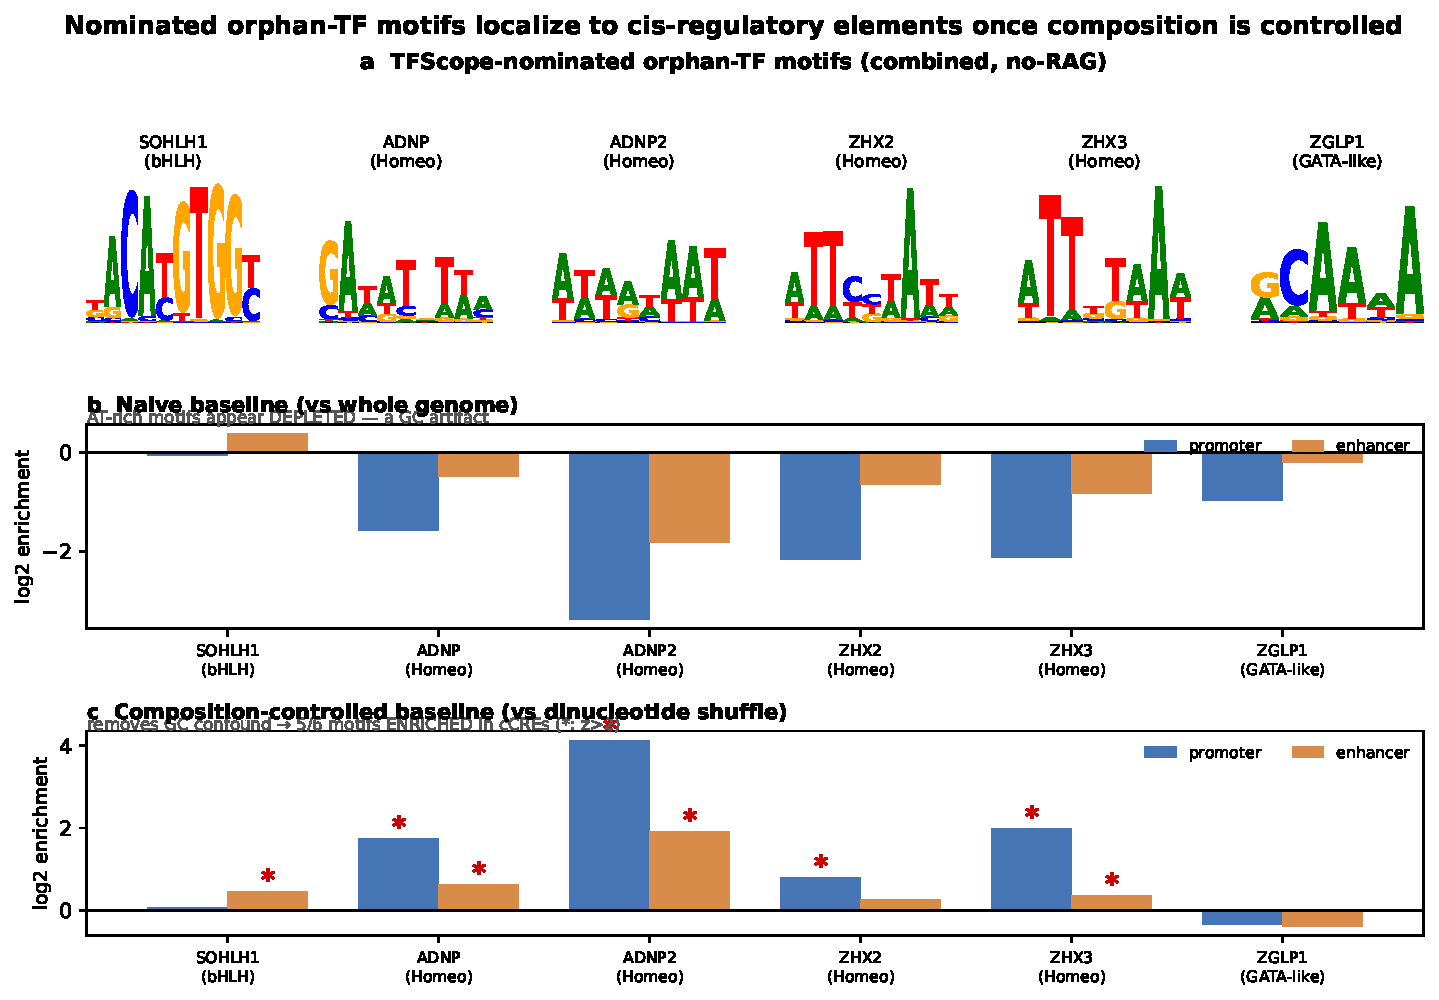
\includegraphics[width=\linewidth]{figures/fig3bc_cre.pdf}\caption{}\end{subfigure}\\[4pt]
  \begin{subfigure}{0.42\linewidth}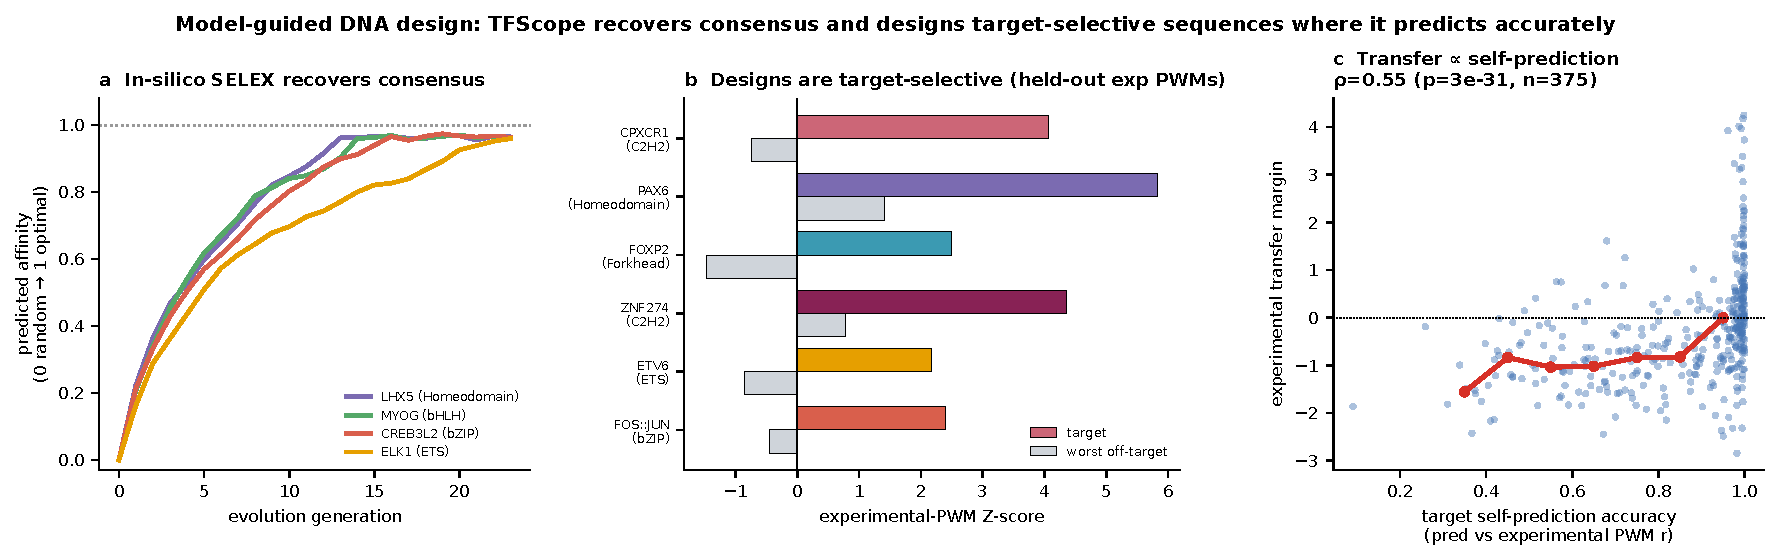
\includegraphics[width=\linewidth]{figures/fig3d_evolution.pdf}\caption{}\end{subfigure}\hfill
  \begin{subfigure}{0.55\linewidth}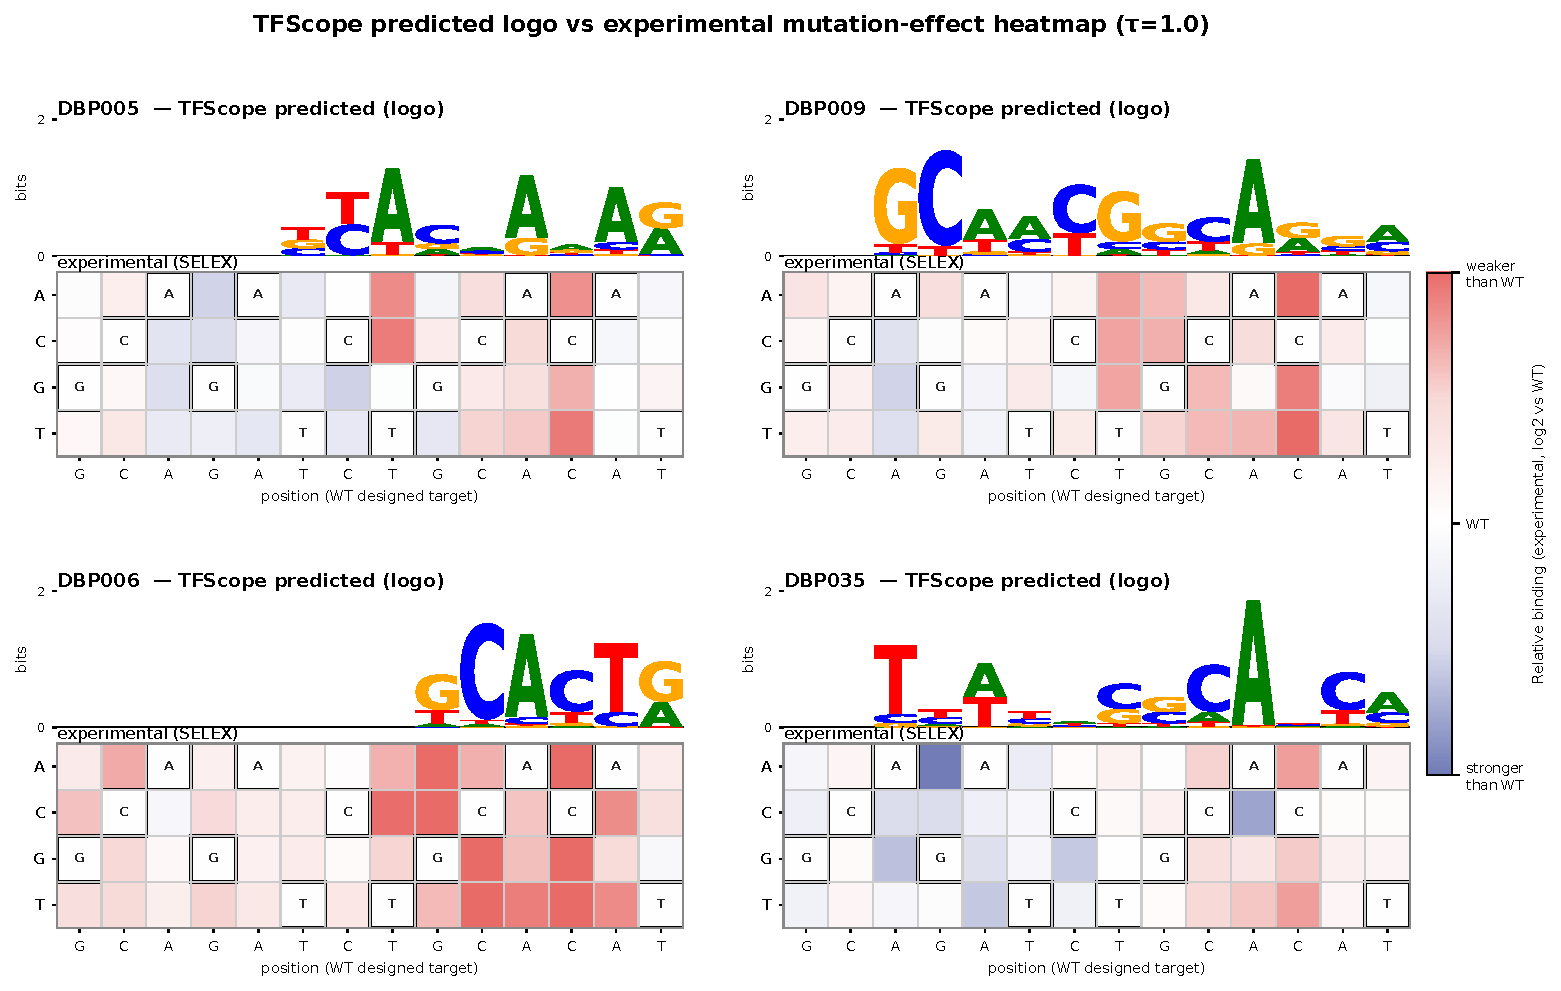
\includegraphics[width=\linewidth]{figures/fig3e_designed.pdf}\caption{}\end{subfigure}
  \caption{\textbf{Proteome-scale specificity for orphan and designed factors.}
  (a) Held-out motif recovery (per-gene median $r$=0.67; 68\% at $r\geq0.5$) declines smoothly with
  DBD identity to training. (b,c) Orphan nominations are enriched in cis-regulatory elements under
  a dinucleotide-shuffle control (5/6 enriched; ADNP2 17.5$\times$ at promoters, SOHLH1 at
  enhancers). (d) Model-guided in-silico DNA optimisation recovers each factor's consensus.
  (e) Sequence-only recovery of de novo designed proteins (DBP5/9/6/35): TFScope predicted logo
  (top) over the experimental mutation-effect heatmap (bottom); the central CAC core is recovered
  with graded confidence (DBP6 $r$=0.65, 83\%; mean 0.53).}
  \label{fig:fig3}
\end{figure}

\begin{figure}[p]\centering
  \begin{subfigure}{0.62\linewidth}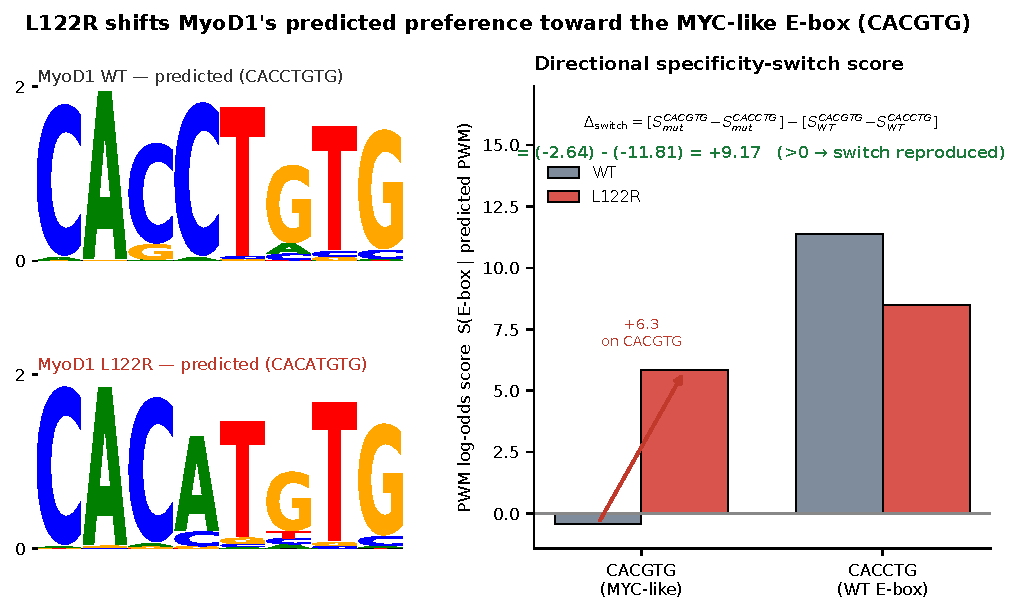
\includegraphics[width=\linewidth]{figures/fig4a_switch.pdf}\caption{}\end{subfigure}\hfill
  \begin{subfigure}{0.36\linewidth}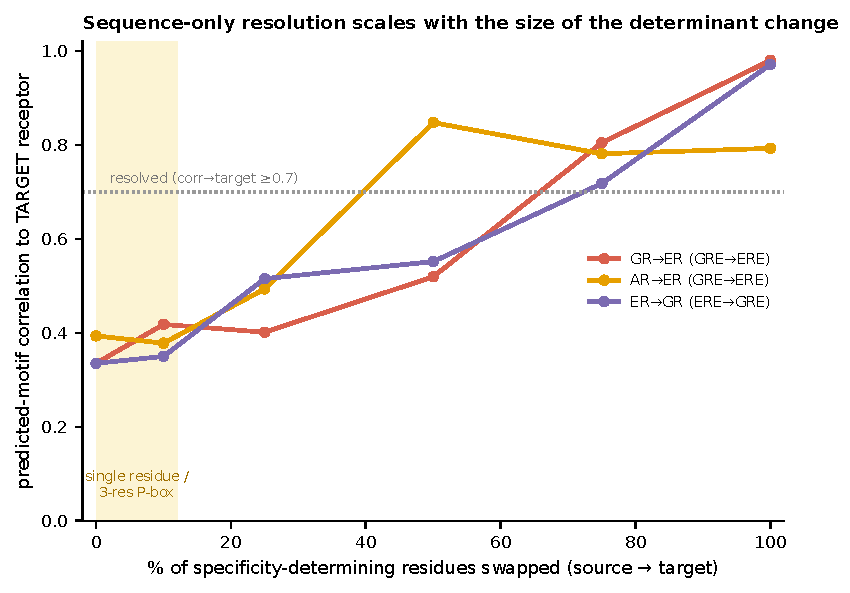
\includegraphics[width=\linewidth]{figures/fig4a_titration.pdf}\caption{}\end{subfigure}\\[4pt]
  \begin{subfigure}{0.7\linewidth}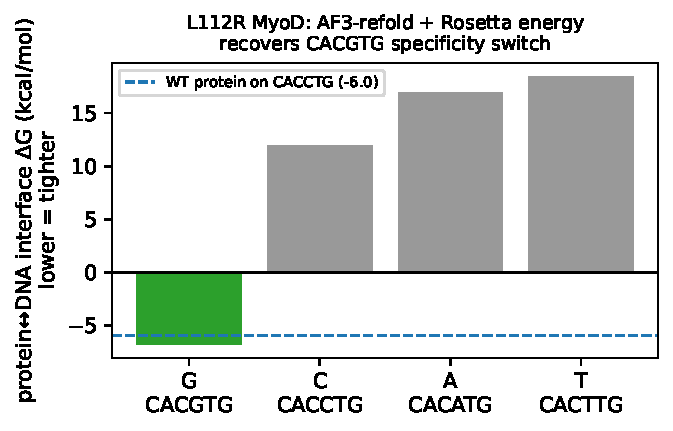
\includegraphics[width=\linewidth]{figures/fig4bc_calibration.pdf}\caption{}\end{subfigure}
  \caption{\textbf{A sequence-to-structure hybrid predicts mutational effects.}
  (a) Directional switch score: MyoD L122R reproduces the documented shift toward the MYC-like
  CACGTG ($\Delta_{\text{switch}}=+9.2$); resolution scales with the number of
  specificity-determining residues swapped (ER$\leftrightarrow$GR P-box / recognition-module
  titration, crossing the resolved threshold at 50--75\%). (b,c) For each candidate base, AF3
  refolds the bHLH dimer and Rosetta scores the interface: by ensemble median CACGTG (G) ranks best
  ($-$25.9 REU) and TFScope's CACATG (A) worst ($-$13.3), calibrating the sequence-only error
  A$\to$G. Sequence localises and scales; structure calibrates the atomic base.}
  \label{fig:fig4}
\end{figure}

\end{document}
